\documentclass[11pt,aspectratio=169]{beamer}

% Style
\usepackage{turnipmetropolis}

% TODOs
\usepackage[nofootnotes,warn]{turniptodo}

\usepackage{graphicx}

% Citations
\usepackage[beamer]{turnipcite}
\bibliography{thesis}
% Numbers in beamer bibliography
\setbeamertemplate{bibliography item}{\insertbiblabel}


\newcommand{\code}[1]{\texttt{#1}}
\newcommand{\citeauthoryear}[1]{\citeauthor{#1}, \citeyear{#1}}

% Get \point, \spoint, \sitem for easy nesting of items
\usepackage{turnippoints}

% Get \twocol, \twostack
\usepackage{turnipbeamerlayout}

\usepackage{booktabs}
\usepackage{array}

\title{Capability-Based Memory Protection for Scalable Vector Processing}
\author{Samuel Stark (\href{mailto:sws35@cam.ac.uk}{sws35@cam.ac.uk})}
\date{June 16th 2022}

\usepackage{multirow}

\begin{document}

\maketitle


%%%%%%%%%%%%%%%%%%%%%%%%%%%%%%%%%%%%%%%%%%%%%%%%%%%%%%%%%%%%%%%%%%%%%%%%%%%%%%%%%%%%%%%%%%%%%%%%%%%%%%%
\metroset{sectionpage=none}
\section{Intro}
\metroset{sectionpage=progressbar}

\begin{frame}{Impenetrable Title}
    \begin{center}
        \Large \alert<2-3>{Capability-Based Memory Protection} for \\\alert<3>{Scalable Vector Processing}
    \end{center}
    \note{
    Utterly impenetrable title
    
    Need to understan both x and y
    
    explain both of these first
    
    project should come along for the ride
    }
\end{frame}

\begin{frame}[t]{Background - What is CHERI?}

\begin{center}
    \Large {Capability-Based Memory Protection} \code{==} \alert{CHERI}\footnote{Capability Hardware Enhanced RISC Instructions\cite{TR-941}}
\end{center}


\begin{itemize}
    \spoint{Memory is normally addressed with integers}
        {Integer addresses can be \emph{forged}
        \item Code can be \alert{tricked} into accessing memory it shouldn't}
        
    \sitem{CHERI architectures use \emph{capability} addressing}
        {Capability = Bounds + current address}
    \item{Capabilities cannot be forged, only \emph{derived} from other capabilities}
\end{itemize}

\begin{center}
    Code can only access memory when it has been \emph{given} access to that memory
\end{center}

\note{
CHERI initiative started at the computer lab

Apply CHERI to processor arch for improved security

Normal archs use integer-addressed memory

"give me byte 500"

Any code can pull "500" out of thin air and access it

The problem is attackers can trick your code into generating "500" and accessing it, even when it shouldn't

for our purposes capabilities = bounds you can access + a specific address in that bounds

hardware makes sure you only access data within capability bounds

hardware makes sure you only derive capabilities from other capabilities

very useful security property
}
\end{frame}

\begin{frame}[t]{Background - What are vectors?}
    \begin{center}
        \Large (Scalable) Vector Processing
    \end{center}

\twocol{0.7}{0.3}{
\begin{itemize}
    \item{Vector architectures allow programmers to use SIMD}
    \spoint{Most vector architectures have \emph{fixed-length} vectors}{SSE, Arm Neon = 128-bit, AVX-512 = 512
    \item Vector lengths have hardware tradeoff
    \item Need to recompile code for different vector lengths}
    \spoint{\emph{Scalable vector} architectures give designers flexibility\cite{stephensARMScalableVector2017}}{Code doesn't rely on fixed vector length}
\end{itemize}
}{
\bgroup
\def\arraystretch{1.2}
\begin{table}[]
    \centering
    \begin{tabular}{|c|c|c|c|}
\hline
24&	9&	9&	28\\
\hline
\multicolumn{4}{c}{\Large +} \\
\hline
13&	17&	10&	24  \\
\hline
\multicolumn{4}{c}{\Large =} \\
\hline
37& 26& 19& 52 \\
\hline
\end{tabular}
    \caption{Vector addition}
\end{table}
\egroup
}

\note {
}
\end{frame}


\begin{frame}{Have we combined them before?}
    \begin{itemize}
        \spoint{CHERI affects vector memory accesses}{Loading N vector elements in a single instruction \item Per-element bounds checks could be expensive?}
    
        % \spoint{Per-element access checks could be \emph{expensive}}{But vectors are too prevalent to ignore}
    
        \spoint{Arm have manufactured CHERI hardware}{Has fixed-length SIMD \item Doesn't support complex access patterns}
        \point{No other general-purpose CHERI processors with vector support}
    \end{itemize}
    
\begin{center}
    Where does this matter?
\end{center}
\end{frame}

\begin{frame}[t]{Background - Where does it matter most?}
\twocol{0.6}{0.4}{
    \begin{center}
        \Large \textbf{\only<2->{Vectorized }\code{memcpy}!}
    \end{center}
    \vfill\null
    \begin{itemize}
        \point{Take data and copy it somewhere else}
        \point{Extremely widespread operation}
        \point{Vectors can copy more data per instruction}
        \point{Vectorized \code{memcpy} should work and go fast on CHERI}
    \end{itemize}
}{
    \only<1>{
    % \begin{figure}
        % \centering
        
\includegraphics[width=\textwidth,height=6.5cm,keepaspectratio]{figures/meme-scalar.jpg}
        % \caption{Scalar \code{memcpy}}
    % \end{figure}
    }
    \only<2>{
    % \addtocounter{figure}{1}
    % \begin{figure}
        % \centering
        
\includegraphics[width=\textwidth,height=6.5cm,keepaspectratio]{figures/meme-vector.jpg}
        % \caption{Vectorized \code{memcpy}}
    % \end{figure}
    }
}


\end{frame}

\begin{frame}[t]{Project goal}

    \begin{center}
        Make vectorized \code{memcpy} functional and fast on CHERI\\
    \end{center}

    \begin{center}
        Combine the RISC-V Vector extension (RVV) with CHERI-RISC-V\\
    \end{center}
    
\only<2>{
\vfill\null
    \begin{columns}[T]
    \centering
\column{0.4\textwidth}
\begin{block}{RVV (original)}
\begin{itemize}
    \item Uses integer addressing
    \begin{itemize}
        \item[]
    \end{itemize}
    \item Loads/stores integer data
\end{itemize}
\end{block}

\column{0.55\textwidth}
\begin{block}{CHERI-RVV (ours)}
\begin{itemize}
    \item Uses \alert{capability} addressing
    \begin{itemize}
        \item Performance concerns?
    \end{itemize}
    \item Loads/stores integers \alert{and capabilities}
    \item Doesn't break CHERI security
\end{itemize}
\end{block}
\end{columns}
\vfill\null
}

\begin{center}
  \begin{minipage}[c]{0.6\linewidth}
  \only<1>{
  \vfill\null
    \begin{enumerate}
        \sitem{Write a RISC-V CHERI-RVV emulator in Rust}{Demonstrates hardware feasibility}
        \sitem{Write test programs in C}{Demonstrates software feasibility}
        \point{Run the test programs on the emulator!}
    \end{enumerate}
}
\end{minipage}
\end{center}

\end{frame}

%%%%%%%%%%%%%%%%%%%%%%%%%%%%%%%%%%%%%%%%%%%%%%%%%%%%%%%%%%%%%%%%%%%%%%%%%%%%%%%%%%%%%%%%%%%%%%%%%%%%%%%
\section{Step 1: Making vector accesses \emph{use} capabilities}

\begin{frame}{Vector memory access patterns}
\twocol{0.4}{0.6}{
% Three patterns for vector memory accesses
\vfill\null
\begin{enumerate}
    \alert<1>{\spoint{Unit-stride}{\code{base, base+1, base+2...}}}
    \alert<2>{\spoint{Strided}{\code{base, base+n, base+2n...}}}
    \alert<3>{\spoint{Indexed}{\code{base + index[0], base + index[1], base + index[2]...}}}
\end{enumerate}
}{
    \only<1>{
    \begin{figure}
        \centering
        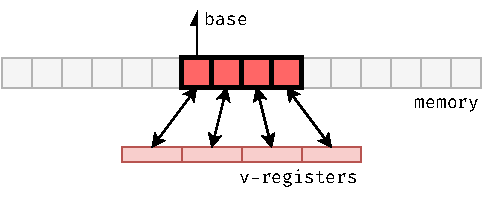
\includegraphics[width=\textwidth,height=6cm,keepaspectratio]{figures/unit.pdf}
        \caption{Unit access}
    \end{figure}
    }
    \only<2>{
    \addtocounter{figure}{1}
    \begin{figure}
        \centering
        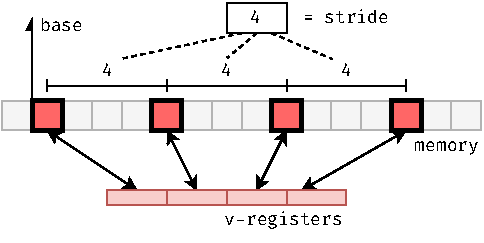
\includegraphics[width=\textwidth,height=6cm,keepaspectratio]{figures/strided.pdf}
        \caption{Strided}
    \end{figure}
    }
        \only<3>{
    \addtocounter{figure}{2}
    \begin{figure}
        \centering
        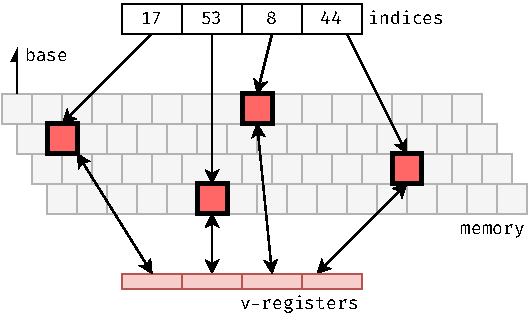
\includegraphics[width=\textwidth,height=6cm,keepaspectratio]{figures/indexed.pdf}
        \caption{Indexed}
    \end{figure}
    }
    }
\end{frame}

\begin{frame}{Vector memory access patterns}
\newcommand{\basetocap}{Base \only<1>{address}\only<2>{\alert{capability}}}
\newcommand{\basetocapaddr}{\only<2>{{\footnotesize \code{0x3700.. }}}\code{0x37f0}\only<2>{{\footnotesize  \code{ ..0x3800}}}}

    \begin{tabular}{p{3cm}>{\centering\arraybackslash}p{6.75cm}>{\centering\arraybackslash}p{3cm}}
    \toprule
    \multicolumn{3}{l}{\textbf{Unit-stride}} \\
    \midrule
    \basetocap{} & \basetocapaddr{} & 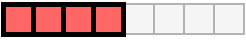
\includegraphics[width=3cm,height=1cm,keepaspectratio]{figures/min-unit.pdf}\\
    
    \midrule
    \multicolumn{3}{l}{\textbf{Strided}} \\
    \midrule
    \basetocap{} & \basetocapaddr{} & \multirow{2}{*}{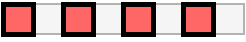
\includegraphics[width=3cm,height=2cm,keepaspectratio]{figures/min-strided.pdf}}\\
    Stride & \code{2} & \\

    \midrule
    \multicolumn{3}{l}{\textbf{Indexed}} \\
    \midrule
    \basetocap{} & \basetocapaddr{} & \multirow{2}{*}{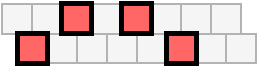
\includegraphics[width=3cm,height=2cm,keepaspectratio]{figures/min-indexed-wide.pdf}}\\
    Index vector & \begin{tabular}{|c|c|c|c|}\hline 8 & 2 & 13 & 4 \\ \hline\end{tabular} \\
    
   \bottomrule
   \rule{0pt}{3ex}
   {\footnotesize Property} & {\footnotesize Example value} & {\footnotesize Memory pattern} 
    \end{tabular}
\end{frame}


%%%%%%%%%%%%%%%%%%%%%%%%%%%%%%%%%%%%%%%%%%%%%%%%%%%%%%%%%%%%%%%%%%%%%%%%%%%%%%%%%%%%%%%%%%%%%%%%%%%%%%%
\section{Step 2: Making vector accesses \emph{copy} capabilities}

\begin{frame}{Storing capabilities in memory}
    \twocol{0.5}{0.5}{
    \begin{itemize}
        \point{Memory can hold both capabilities and integers}
        \spoint{Separate \emph{tag memory} denotes which regions are capabilities}{Access to tag memory is controlled by hardware}
        \point{Without the tag, you get the \emph{integer encoding} of the capability}
    \end{itemize}
    }{
    \only<1>{
    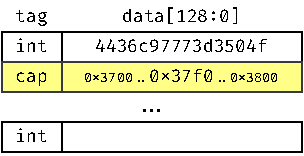
\includegraphics[width=\textwidth,height=6cm,keepaspectratio]{figures/mem-tagged.pdf}
    }
    \only<2>{
    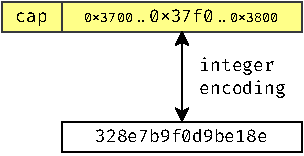
\includegraphics[width=\textwidth,height=6cm,keepaspectratio]{figures/mem-intencode.pdf}
    }
    }
\end{frame}

% \begin{frame}{Integer-only \code{memcpy}}
% \twostack{
% \vfill\null
%     \only<1>{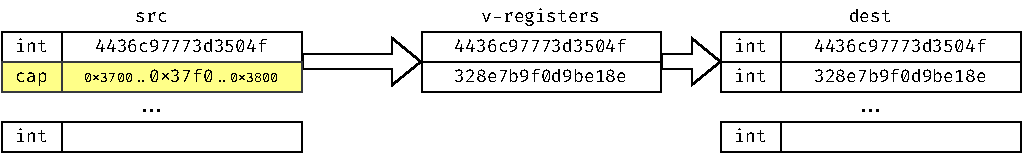
\includegraphics[width=\textwidth,height=6cm,keepaspectratio]{figures/memcpy-tagless.pdf}}
%     \only<2>{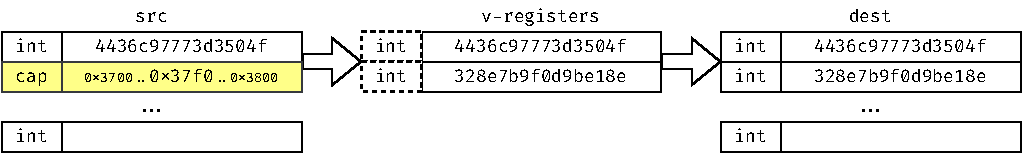
\includegraphics[width=\textwidth,height=6cm,keepaspectratio]{figures/memcpy-implicitint.pdf}}
%     }{
%     \begin{itemize}
%         \point{The original RVV specification doesn't consider capabilities}
%         \point{Assumes vectors only hold \alert{integer} data}
%         \point{$\Rightarrow{}$ \code{memcpy} converts capabilities to integers :(}
%     \end{itemize}
%     }
% \end{frame}

% \begin{frame}{Copying capabilities in vectors}
% \twostack{
%     \vfill\null
%     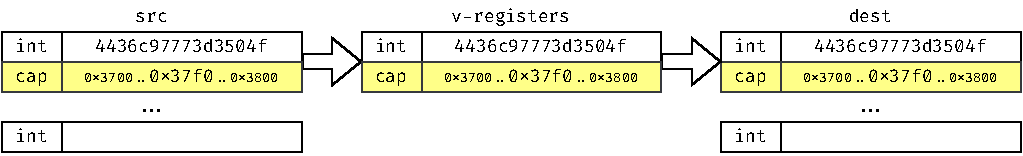
\includegraphics[width=\textwidth,height=6cm,keepaspectratio]{figures/memcpy-tagged.pdf}
%     }{
%     \begin{itemize}
%         \point{If we add tag bits to vector registers, we can load/store them correctly}
%         \spoint{But does that make anything else more complicated?}{Yes}
%     \end{itemize}
%     }
% \end{frame}

\begin{frame}{Integer-only \code{memcpy}}
\twocol{0.6}{0.4}{
    \begin{itemize}
        \point{The original RVV specification doesn't consider capabilities}
        \point{Assumes vectors only hold \alert{integer} data}
        \point{$\Rightarrow{}$ \code{memcpy} converts capabilities to integers :(}
    \end{itemize}
    }{
\vfill\null
    \only<1>{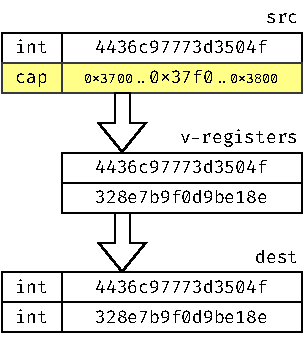
\includegraphics[width=\textwidth,height=6cm,keepaspectratio]{figures/memcpy-tagless-vertical.pdf}}
    \only<2>{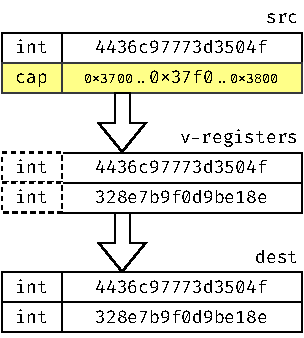
\includegraphics[width=\textwidth,height=6cm,keepaspectratio]{figures/memcpy-implicitint-vertical.pdf}}
    }
\end{frame}

\begin{frame}{Copying capabilities in vectors}
\twocol{0.6}{0.4}{
    \begin{itemize}
        \point{If we add tag bits to vector registers, we can load/store them correctly}
        \spoint{But does that make anything else more complicated?}{Yes}
    \end{itemize}
    }{
    \vfill\null
    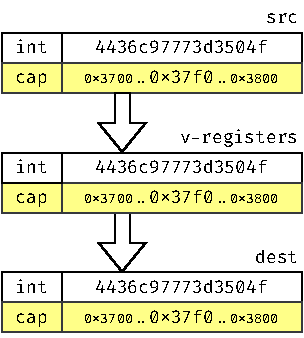
\includegraphics[width=\textwidth,height=6cm,keepaspectratio]{figures/memcpy-tagged-vertical.pdf}
    }
\end{frame}

\begin{frame}{\emph{Storing} capabilities in vectors???}
    \twocol{0.5}{0.5}{
\begin{itemize}
    \point{Now \emph{all vector instructions} can interact with capabilities!}
    \point{If we aren't careful, attackers could forge capabilities}
    \spoint{We introduce two contexts of accessing vector registers}{Integer context \item Capability context}
\end{itemize}}{
\only<1>{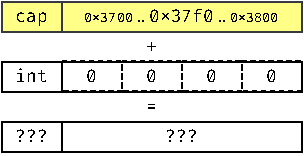
\includegraphics[width=\textwidth,height=6cm,keepaspectratio]{figures/vadd-cap-unk.pdf}}
\only<2>{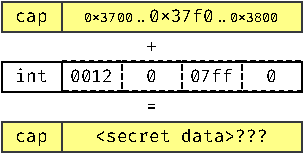
\includegraphics[width=\textwidth,height=6cm,keepaspectratio]{figures/vadd-cap-badcap.pdf}}
\only<3>{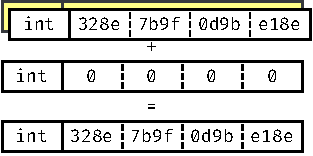
\includegraphics[width=\textwidth,height=6cm,keepaspectratio]{figures/vadd-cap-int.pdf}}
}
\end{frame}

\begin{frame}{Integer/Capability context}
    \twocol{0.5}{0.5}{
        \begin{center}
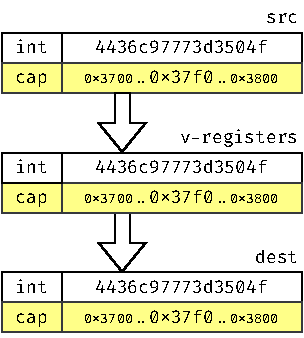
\includegraphics[width=\textwidth,height=6cm,keepaspectratio]{figures/memcpy-tagged-vertical.pdf}
        Capability context\\(128-bit vector loads/stores)
    \end{center}
    }{
        \begin{center}
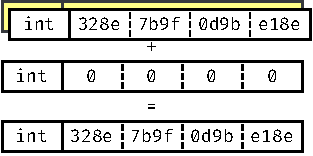
\includegraphics[width=\textwidth,height=6cm,keepaspectratio]{figures/vadd-cap-int.pdf}
        Integer context\\(Everything else)
    \end{center}
    }
\end{frame}

\begin{frame}{\code{memcpy} works!}
    \begin{tabular}{lcccccc}
\toprule
& RV32 & \multicolumn{5}{c}{RV-64} \\
\cmidrule(lr){2-2} \cmidrule(lr){3-7}
& \code{llvm-13} & \code{llvm-13} & \code{llvm-15} & \code{gcc} & CHERI & CHERI (Int) \\
\midrule
Copy & Y & Y & Y & Y & Y & Y\\
Copy + Invalidate & - & - & - & - & Y & Y\\
\bottomrule
    \end{tabular}
\end{frame}

%%%%%%%%%%%%%%%%%%%%%%%%%%%%%%%%%%%%%%%%%%%%%%%%%%%%%%%%%%%%%%%%%%%%%%%%%%%%%%%%%%%%%%%%%%%%%%%%%%%%%%%
\metroset{sectionpage=none}
\section{Conclusion}
\metroset{sectionpage=progressbar}

\begin{frame}{Conclusion}
    \twocoltop{0.6}{0.4}{
    \begin{block}{CHERI-RVV Summary}\vspace{0.1em}
    \begin{tabular}{l}
        \toprule
        Uses capability addressing \\
        Loads/stores integers and capabilities \\
        Doesn't break CHERI security \\
        \midrule
        Supports all vanilla RVV instructions \\
        \alert<2>{Is binary-compatible with vanilla RVV} \\
        \alert<2>{Can be* source-compatible with vanilla RVV} \\
        \midrule
        Has a reference implementation: \\
        Emulator, compiler*, test programs \\
        9,500 LoC \\
        \bottomrule
        *compiler requires engineering work \\
    \end{tabular}
    \end{block}
    }{
    \begin{block}{Future work}
\vspace{0.5em}
Do more with vectors than just
\begin{enumerate}
    \item Vectorized \code{memcpy}
    \item Vectorized tag clearing
\end{enumerate}

Add new instructions for e.g. temporal revocation\cite{xiaCHERIvokeCharacterisingPointer2019}?

\end{block}
\vspace{3.2em}
\begin{center}
    Samuel Stark\\\href{mailto:sws35@cam.ac.uk}{sws35@cam.ac.uk}
\end{center}%
}
    
\end{frame}

\appendix
\begin{frame}{Per-element checks}
    \begin{itemize}
        \spoint{Vector hardware can coalesce element accesses}{e.g. 4x 32-bit elements in the same cache line can be transferred over a 128-bit bus at once}
        \spoint{Want to coalesce the per-element capability checks as well}{Otherwise they could bottleneck \item Or use too much logic}
        \spoint{We found we \emph{can} coalesce capability checks if they succeed}{i.e. "is the cache line inside the capability bounds" \item But if that check fails, we have to check each element individually \item RVV requires that any synchronous exception (i.e. capability check) reports the element that triggered it}
    \end{itemize}
\end{frame}

% References slide
\turnipbibframe{}

% Appendix slides here

\end{document}
